\subsubsection{Unfolding of the matrix power}
\label{sec:unfolding}
The final  prime function is called monotone unfolding. The general idea is that unfolding unpacks a representation of several trees inside a single tree.  Before describing this function in more detail,  we introduce some notation,  inspired by the matrix power in  universal algebra~\citep[p.~268]{Taylor1975}. 
\begin{definition}
    [Matrix power] For $k \in \set{1,2,\ldots}$ define the $k$-th matrix power of a ranked set $\rSigma$, denoted by $\mati k \rSigma$, to be the ranked set $\reduce k \powersmall \rSigma k$.
\end{definition}
Here is a picture of elements in the third matrix power:
\mypic{102}
% We use the name \emph{registers} for the coordinates $1,\ldots,k$ in the $k$-th matrix power. This terminology will be motivated later on in the paper, where the coordinates of the matrix power will correspond to registers in transducer. 


\begin{figure}[]
    \mypic{101}    
    \caption{Unfolding the matrix power}
    \label{fig:unfold}
\end{figure}

An element of the $k$-th matrix power  can be seen as having a group of $k$ incoming edges, and each of its ports  can be seen as a group of $k$ outgoing edges. The \emph{general unfolding} operation, which has type
\begin{align*}
    \ranked{\tmonad \mati k{\Sigma} \to \mati k{( \tmonad \Sigma)}},
\end{align*}
matches the $k$ incoming edges in a node with the $k$ outgoing edges in the parent port; it also removes the unreachable nodes. This operation is illustrated in Figure~\ref{fig:unfold}, and  a formal definition  is  in the appendix.
% There are two variants of the unfolding operation:
% \begin{align*}
%     \underbrace{\ranked{\tmonad \mati k{\Sigma} \to \mati k{( \tmonad \Sigma)}}}_{\text{general unfolding}} \qquad 
%     \underbrace{\ranked{\tmonad \mati k{\Sigma} \to \termset + \mati k{( \tmonad \Sigma)}}}_{\text{monotone unfolding}} 
%     \end{align*}   




% For an element of the matrix power
% \begin{align*}
% a =    \tensorpair{a_1,\ldots,a_k}/f \in \mati k \rSigma,
%     \end{align*}
% define its \emph{rewiring function} to be  the function
%     \begin{align*}
%     \coprod_{i \in \set{1,\ldots,k}} \text{ports of $a_i$} \quad \to \quad  \underbrace{\text{(ports of $a$)} \times \set{1,\ldots,k}}_{\text{sub-ports of $a$}}
%     \end{align*}
% which is obtained by first interpreting of $a_i$ as one of the ports in the tensor tuple $\tensorpair{a_1,\ldots,a_k}$, and then applying the grouping function $f$. Here is a picture:
% \begin{center}
%     (todo picture)
% \end{center}
% For a node $v$ of the term $t$ and $i \in \set{1,\ldots,k}$, define the $i$-th sub-node of $v$ to be the pair  $(v,i)$. We define a tree structure on sub-nodes as follows. Let   $(v,i)$ be a sub-node, and let $a_i \in \rSigma$ be the $i$-th component in the label of node $v$.  The arity of the sub-node $(v,i)$ is inherited from $a_i$, and its children are defined as follows. Take a port $x \in \set{1,\ldots,\text{arity of $a_i$}}$.  Apply the rewiring function to $(i,x)$, yielding a pair $(j,y)$. Take the $y$-th child of node $v$, call it $w$. The $x$-th child of $(v,i)$ is defined to be $j$-th sub-node of the $y$-th child of $v$.

% The unfolding of $t$ is  defined using the above tree structure. For $j \in \set{1,\ldots,k}$, the root of $t_i$ is the $i$-th sub-node of the root of $t$. The nodes in $t_i$ are all of the sub-nodes of $t$ that can be reached from this root by the child relation defined above, with the corresponding tree structure. Finally, 
\paragraph*{Chain logic.}
The general unfolding operation is too powerful  to be included in the derivable functions, as we explain below. It does, however, admit a characterisation in terms of a fragment of \mso called \emph{chain logic},  see~\cite[Section 2]{thomas1992} or~\cite[Section 2.5.3]{bojanczykDecidablePropertiesTree2004}, whose expressive power is strictly between first-order logic and \mso. Chain logic is defined to be the fragment of  \mso where set quantification is restricted to sets  where all nodes are comparable by  the descendant relation. 

\begin{theorem}\label{thm:chain-transductions}
    The following conditions are equivalent for tree-to-tree functions:
\begin{itemize}
    \item is derivable, as in Definition~\ref{def:derivable-function}, except that general unfold is used instead of monotone unfold;
    \item is a transduction,  as in  Definition~\ref{def:fo-transduction},  except that chain logic is used instead of first-order logic. 
\end{itemize}
\end{theorem}

\begin{figure}
    \mypic{108}
    \caption{Non-monotone unfolding}
    \label{fig:non-monotone}
\end{figure}



 To see why chain logic is needed to describe general unfolding, consider the unfolding in Figure~\ref{fig:non-monotone}, where two coordinates are swapped in each node of the input tree.
For inputs with an odd number of swaps, the output of unfolding has a white leaf in the first coordinate, and for inputs with an even number of swaps, the output has a white leaf in the first coordinate.  Checking if a path has even length can be done in chain logic, but not in  first-order logic.  

% On trees, first-order logic is strictly less expressive than chain logic, which is strictly less expressive than \mso, see~\cite[Fact 2.5.8]{bojanczykDecidablePropertiesTree2004}, and the same inclusions carry over to tree-to-tree transductions.
\paragraph*{Monotone unfolding}
To avoid the problems with cyclic swaps, we impose a monotonicity requirement on the matrix power. 

% instead of general unfold, the prime functions in Figure~\ref{fig:not-explained} use a partial operation of type
% \begin{align*}
%     \ranked{\tmonad \mati k{\Sigma} \to \mati k{( \tmonad \Sigma)} + \termset} ,
% \end{align*}
% which is called \emph{monotone unfolding}. This is the same as general unfolding, except that it is defined only for inputs which satisfy a monotonicity restriction that is explained below.

 Let  $a \in \mati k \rSigma$ be an element of the matrix power,  let $p,q \in \set{1,\ldots,k}$, and let  $i$ be a port of $a$. We write $
     q \to_i p$
if coordinate $q$ in the $i$-th outgoing edge  is connected to  coordinate $p$ in root, as described in the following picture:
\mypic{109}
One can see that $\to_i$ is a partial function from $\set{1,\ldots,k}$ to $\set{1,\ldots,k}$. We call it the  \emph{twist function of the $i$-th port}. For example, the twist function in of the unique port in 
\mypic{110}
swaps coordinates $1$ and $2$.  Call  an element of the matrix power  \emph{monotone} if for every port, its twist functions is monotone (when restricted to inputs where it is defined). The \emph{monotone unfolding} operation in Figure~\ref{fig:unfold} defined to be the restriction of general unfolding,  which  is undefined if the input contains at least one label which is non-monotone, and otherwise returns the output of the general unfolding.

\paragraph*{Is unfolding derivable?} The  prime functions in our main theorem  are meant to be simple syntactic rewritings. It is debatable whether the  unfolding operation -- even in its monotone variant -- is of this kind. For example, proving that monotone unfolding is a first-order transduction requires non-trivial effort, including an invocation of the Sch\"utzenberger-McNaughton-Papert theorem about first-order logic on words being the same as counter-free automata. 

Is it possible to break down monotone unfolding into simpler primitives?
In the appendix, we devote considerable resources to answering this question. We propose one new  datatype
% \begin{align*}
% \shallowterm \rSigma \rGamma \quad \eqdef   \quad \ranked{\coprod_{\black{a \in} \rSigma} } \overbrace{\ranked{\Gamma \product \cdots \product \Gamma},}^{\text{arity of $a$ times}}
% \end{align*}
% which represents trees of depth two, 
and seventeen additional prime functions, which can be called syntactic rewriting without straining the reader's patience. Then, we show that monotone unfolding can be derived using   the new datatype and functions. The proof of this result is one of the main technical contributions of this paper.
% Suppose that the input is 
% \begin{align*}
% (\tensorpair{a_1,\ldots,a_k}/f)\tensorpair{t_1,\ldots,t_n} \in 
% \end{align*}
% First apply the unfold operation to the smaller trees $t_1,\ldots,t_n$, yielding trees
% \begin{align*}
% \tensorpair{t_{11},\ldots,t_{1k}}/f_1 \quad \cdots \quad  \tensorpair{t_{n1},\ldots,t_{nk}}/f_n
% \end{align*}
% For $i \in \set{1,\ldots,k}$ construct a term $s_i$ as follows. The root label is $a_i$. If the arity of $a_i$ is $n_i$, then let $t_{ij}$ be the tree 
% For two ranked sets $\rSigma$ and $\rGamma$, define 
% \begin{align*}
% \shallowterm \rSigma \rGamma \quad \eqdef   \quad \ranked{\coprod_{\black{a \in} \rSigma} } \overbrace{\ranked{\Gamma \product \cdots \product \Gamma}}^{\text{arity of $a$ times}}
% \end{align*}
% \begin{align*}
%     \ranked{
%         \xymatrix{
%             \shallowterm{\mati k \rSigma} {\mati k \rGamma}  \ar[r] & \mati k {(\shallowterm \Sigma \Gamma)}.
%         }
%     }
% \end{align*}
% \begin{align*}
% \tmonad \rSigma = \redset{ \portletter} + \shallowterm \rSigma {\tmonad \rSigma}
% \end{align*}


% to be the set of terms over alphabet $\rSigma + \rGamma$, where the 
% % , this operation of determining the dependency tree is what we call \emph{unfolding}. We illustrate it by the following example 
% % \begin{center}
% % 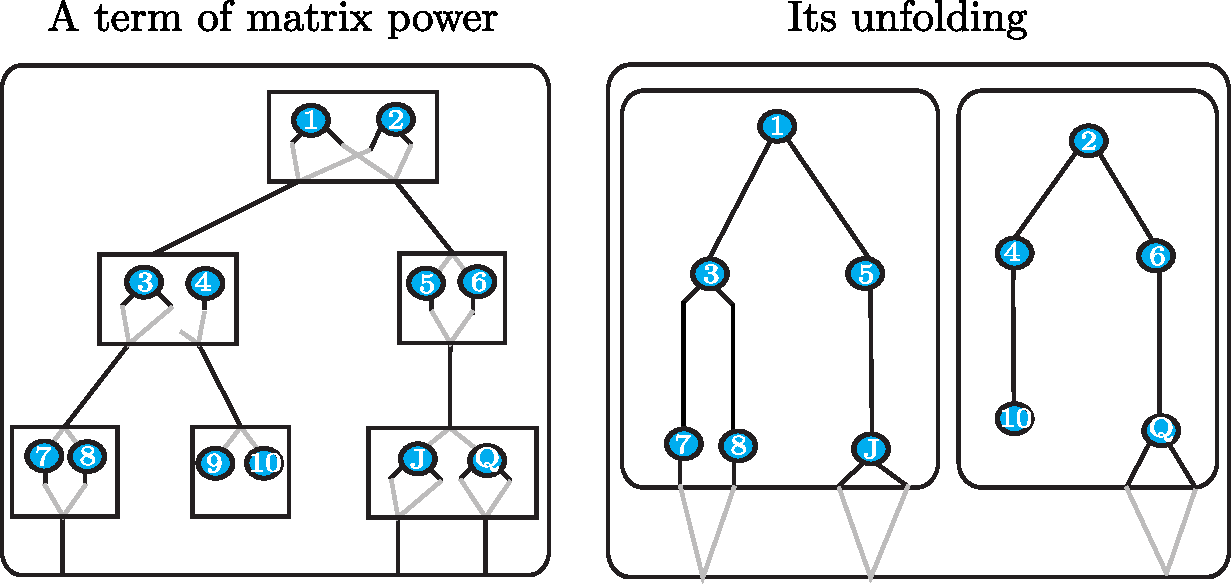
\includegraphics[scale=.38]{unfold-matrix-power}
% % \end{center}
% %  which is defined as follows by induction on the size of the input term. 
% If the input is an empty term, then the output is this term:
% \begin{center}
% \includegraphics[scale=.3, page=83]{pics.pdf}
% \end{center}
% % Otherwise, if the input is a nonempty term $(a_1,\ldots,a_k)/f)(t_1,\ldots,t_n)$. 
% Apply unfolding inductively, yielding 
% For $i \in \set{1,\ldots,k}$ define $s_i$ to be the tree where the root label is $a_i$, and the children are obtained ... 

% Consider an edge in the tree $t$, which connects either a node with one of its children, or a node with one of the ports. For $i \in \set{1,\ldots,k}$, define the $i$-th source of the edge to be the node ; likewise define the $i$-th target of the edge to be the $i$-th subnode of $s$.  For a node $x$ in $t$ and $i \in \set{1,\ldots,k}$, define the $i$-th subnode of $x$ to be the label (from $\rSigma$) in the $i$-th coordinate of the label of $x$.  For a subnode, define its \emph{outgoing edge} to be the edge of the tree 

% Define a \emph{inport} of $s$ to be a pair (node of $s$, number in $\set{1,\ldots,k$}). Define an \emph{outport} to be a pair (node $s$, number in $\set{1,\ldots,k}$, number in $\set{1,\ldots,\text{arity of $s$}$}). 

% \begin{align*}
% \underbrace{\text{(nodes in $s$)} \times \set{1,\ldots,k}}_{\text{sub-nodes}} 
% \qquad
% \underbrace{\text{(edges in $s$)} \times \set{1,\ldots,k}}_{\text{sub-edges}}
% \end{align*}
% For a sub-node $(v,i)$, define its label to be the label in $\rSigma$ of the $i$-th coordinate in the label of $v$. Define the arity of the sub-node to be the arity of its label. If a sub-node has arity $n$, and $j \in \set{1,\ldots,n}$, then the $j$-th out-going sub-edge of the sub-node is defined in the natural way. 


% Consider an  element
% \begin{align*}
% (a_1,\ldots,a_k)/f  
% \end{align*}

% \begin{align*}
% \coprod_{i \in \set{1,\ldots,k}} \set{1,\ldots,\text{arity of $a_i$}} \qquad \to \qquad \set{1,\ldots,n} \times \set{1,\ldots,k}
% \end{align*}
% For $i \in \set{1,\ldots,k}$ and a node node $v$ in the tree $s$ which has label $(a_1,\ldots,a_k)/f$. For $j \in \set{1,\ldots,\text{arity of $a_i$}}$. Let define the $j$-th child of to be the 

% Define a \emph{sub-edge} to be a pair (edge in $s$, number in $\set{1,\ldots,k}$). Define a \emph{sub-node} to be a pair (node in $s$, number in )

% then the output is obtained by first applying unfolding to to the smaller terms $t_1,\ldots,t_n$, and then applying the following derivable function, which we call \emph{shallow unfold}. 
% \begin{align*}
%     \ranked{
%         \xymatrix{
%             \shallowterm{\mati k \rSigma} {\mati k \rGamma}  \ar[r] & \mati k {(\shallowterm \Sigma \Gamma)}.
%         }
%     }
% \end{align*}
% Here is a picture of unfolding for shallow terms:
% \begin{center}
% 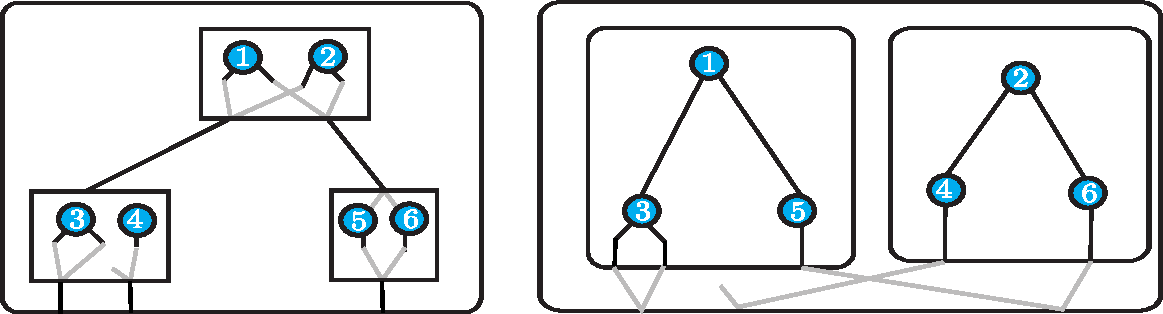
\includegraphics[scale=.4]{unfold-shallow}
% \end{center}